\chapter{Introduction}
\label{sec:introduction}

The work in this thesis is concerned with the analysis of the rhythmic structure in performances of music. We will study rhythmic structure in isolation of other structures that may be present in the music like melody or harmony.

This chapter will introduce concepts used throughout this thesis and discuss related studies. First, rhythmic structure is introduced. Then in section \ref{sec:performances}, structure will be related to performance and finally in section \ref{sec:introducing} the approach presented in this thesis will be introduced.

The rest of this thesis is structured as follows: In chapter \ref{sec:method}, our approach will be described in detail. Chapter \ref{sec:method} will also introduce the annotated jazz corpus that was produced for this thesis. In chapter \ref{sec:evaluation}, we will describe how we intend to evaluate our system. Then in chapter \ref{sec:results} the system will be evaluated on the jazz corpus. Chapter \ref{sec:discussion} will discuss to what extent the system was successful based on the results and improvements will be suggested. Finally, chapter \ref{sec:conclusion} will present the conclusions of this thesis.

\section{Rhythmic Structure}
\label{sec:structure}

In most Western music traditions, a rhythm is constructed of notes and rests with some metrical duration. A note tells the performer to play some pitch for the duration of the note, a rest indicates a silence for the duration of the rest. A metrical duration can be subdivided into a prime number of beats. The first of these beats is called the \textit{downbeat}, the rest are called \textit{upbeats}.

In the so-called staff notation, metrical units have been given names and durations are specified as subdivisions of the duration of what is called a whole note: half notes or rests, quarter notes or rests, eighth notes or rests, etcetera. Their notation is shown in figure \ref{fig:notation}. Apart from these duple divisions, triple, quintuple and any other prime number divisions are allowed as well. These divisions are called tuplets. Duple and triple divisions are by far the most common in Western music.

\begin{figure}
\centering
\begin{tabular}{lllll}
\parbox{0.15\linewidth}{
\centering
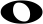
\includegraphics[scale=0.5]{img/whole_note}
}
&
\parbox{0.15\linewidth}{
\centering
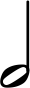
\includegraphics[scale=0.5]{img/half_note}
}
&
\parbox{0.15\linewidth}{
\centering
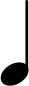
\includegraphics[scale=0.5]{img/quarter_note}
}
&
\parbox{0.15\linewidth}{
\centering
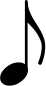
\includegraphics[scale=0.5]{img/eighth_note}
}
&
\parbox{0.15\linewidth}{
\centering
\includegraphics[scale=0.5]{img/meter}
}
\\
A whole note. & A half note. & A quarter note. & An eighth note & A 4/4 time signature\\

\end{tabular}
\caption{Some music notation conventions.}
\label{fig:notation}
\end{figure}

Metrical durations are grouped together in units called bars or measures. A \textit{time signature} specifies how a bar is subdivided into metrical units. The time signature consists of two numbers written above each other. A 4/4 time signature is shown on the far right in figure \ref{fig:notation}. The top number specifies the number of beats per measure, the bottom number specifies the units of those beats. The time signature is sometimes called meter.

Staff music notation is one of the most widespread representations of rhythmic structure. In the field of rhythm analysis, another structure is popular, called a \textit{metrical grid}, originally introduced by \citet{lerdahl1983generative} in their Generative Theory of Tonal Music. A metrical grid is a representation that contains several levels. The lowest level corresponds to the smallest subdivision and the highest level corresponds to a bar. Going down one level corresponds to a subdivision. A metrical grid representing a 3/4 time signature is shown in figure \ref{fig:grid}. Bars are separated using a vertical line, $\bullet$ symbols indicate the downbeats of each level. Level three for example contains one downbeat per bar. Level three is subdivided into three level-two downbeats, the second and third of which is a level-three upbeat. Every level-two unit is subdivided into two level-one downbeats, the second of which is a level-two upbeat. The time signature specifies that a bar is divided into three quarter notes, so level two corresponds to quarter notes in this case.

\begin{figure}[b]
\centering
\hspace{2in}
\setlength{\extrarowheight}{-10.5pt}
\begin{tabular}{llllll|llllll|ll}
$\bullet$ &  &  &  &  &  & 		$\bullet$ &  &  &  &  &  & $\bullet$ & Level 3\\ 
$\bullet$ &  & 	$\bullet$ &  & 	$\bullet$ & & 	$\bullet$ & & $\bullet$ &  & $\bullet$ &  & $\bullet$ & Level 2\\
$\bullet$ & 		$\bullet$ & 		$\bullet$ & 		$\bullet$ & $\bullet$ & $\bullet$ & $\bullet$ & $\bullet$ & $\bullet$ & $\bullet$ & $\bullet$ & $\bullet$ & $\bullet$ & Level 1\\
\end{tabular}
\caption{Metrical grid of a 3/4 time signature.}
\label{fig:grid}
\end{figure}

Having now introduced two representations of rhythmic structure, we can turn to some of the work done in this field. The most extensive recent study was conducted by \cite{temperley2010modeling}, who studied the probabilistic properties of rhythmic structures in isolation from melody and harmony. It is suggested that rhythm has some probabilistic characteristics that are shared to some extent by rhythms in a wide range of musical styles. Temperley identifies a number of intuitions about rhythm that seem to be common practice. These intuitions include the general tendency of onsets to fall on downbeats, the preference for onsets on upbeats to be preceded or followed by a note on the previous or next downbeat and the tendency of long notes to fall on downbeats. 

Temperley compares six different models intended to be sensitive to these regularities. The adequacy of these models is evaluated by measuring their cross-entropy, using cross-validation on a corpus of European folk songs. Temperley's work shows that probabilistic models can successfully differentiate sensible rhythms from nonsensical rhythms. Intuitively, these models explain that not every pattern of onsets that can be described as a valid rhythmic structure will be perceived as a rhythm by humans. 

% Metrical grids?

\section{Performances}
\label{sec:performances}

Rhythmic structure in itself does not define the absolute timing of notes. The common way to relate a rhythmic structure to a performance is by assigning some real duration to a metrical unit. The amount of real time we assign to a metrical duration is usually called the \textit{tempo}. Given a tempo, a rhythmic structure can be converted to a set of \textit{idealised} onset times, also called \textit{metronomic} onset times. Onset times are the time at which a performer started playing a note, measured from the beginning of the performance.

When humans perform a rhythm, they deviate from the idealised onset times in several ways. Unless a metronome is used, the tempo will usually fluctuate as the performance progresses. Much of this fluctuation is intentional and is referred to as \textit{musical expression}. Apart from global tempo changes humans deviate from idealised onsets locally as well, even when a metronome is used. 

In general, it is thought that, depending on the competence of the performer, some proportion of this local deviation, is noise but a large proportion of it seems to be systematic. A study by \citet{palmer1989mapping} suggested that global tempo changes are mostly guided by conscious intention. Local deviations in timing and loudness seemed to be partly unconscious and represented in the performers mind in abstracted form. Pianists were for example aware that they articulated certain beats but could not reliably tell whether they did so by playing them louder or by altering their timing. These findings suggest that it is to some extent not even possible for a human to perform rhythm without expression.

It seems thus that whereas global tempo changes may be guided by conscious intentions of phrasing, local expression may be partially unconscious and unavoidable. Another study has shown that there is some regularity in local expression that is linked to rhythmic structure \citep{bengtsson1983analysis}. For example in Vietnamese waltzes, which have almost exclusively a 3/4 or 6/8 meter, it is observed that there is a consistent lengthening of the first upbeat at quarter note level.

Although a performance deviates from the idealised onsets given by the structure and tempo, human listeners are often able to perceive the rhythmic structure in a performance and multiple listeners tend to be quite consistent in their structural interpretations of a performance. In fact, the studies mentioned earlier suggest that deviations from idealised onsets are crucial to perception of structure in rhythm.

%Much of this expression appears to be a highly complicated and irregular process that is influenced by factors as musical style and the `mood' of the music, the audience and the performer. There is a field of research concerned with finding models for musical expression, see for example \citet{widmer2004computational}. Here, we will not concern ourselves with extensive models of expression. Instead, we will suggest that there may be more regular forms of local expression that are the result of a tendency of humans to emphasize downbeats.

Several authors have suggested models that try to mimic this human capacity. \citet{cemgil2000rhythm} propose a system for rhythm quantisation that uses Bayesian modelling to derive the rhythmic structure. Their model tries to optimise the probability of a score given a performance, which can be expressed as the probability of the score (the score model) times the probability of the score given the performance (the rhythm model). The model assumes tempo can change and uses a tempo-track (often called tempo-curve) to derive metronomic onset times given local tempo. Their performance model simply penalises performances to the extent that they deviate from metronomic onset times. 

\citet{raphael2002hybrid} proposes another model that is similar to the model of \citet{cemgil2000rhythm}. Here a graphical probabilistic model is proposed where `score-positions' (relative positions of notes within a measure) are seen as a Markov chain of events where the probability of a score-position depends on the probability of a note on that score-position and the probability of a note on that score-position preceded by the score-position of the previous note. Another Markov chain of tempo values is generated from the the score positions and finally the exact onset time of each note is dependent on the tempo value, score position of the previous note and score position of the current note.

These models are discussed by \citet{temperley2007music} and it is observed their representation of rhythm is still ambiguous with respect to meter. Temperley proposes a model of rhythm that is based on a metrical grid, an unambiguous representation of meter and also contains fewer parameters than the rather complicated models of \citet{raphael2002hybrid} and \citet{cemgil2000rhythm}. This model is elaborated in \citet{temperley2009unified} where it is integrated into a unified probabilistic model of rhythm, harmony and polyphonic structure.

In the latter study, a rhythm model is implemented based on a concept that Temperley calls metrical anchoring: the probability of a note on an upbeat depends on whether a note was played on the preceding or following downbeat. Temperley calls this model the hierarchical position model. Later, in \citet{temperley2010modeling}, this model is compared to other rhythm models and it is shown that it performs well in comparison. 

The hierarchical model uses metrical grids as a representation of rhythm. These grids are limited to four levels and contain only duple divisions. To deal with the problem of tempo, the model has a parameter that specifies the preferred \textit{tactus level} interval. The tactus level corresponds to the tactus, or pulse, in a performance which often corresponds to quarter notes. The tactus interval is allowed to fluctuate: the probability of a next tactus interval is a normal distribution over the previous one, preferring tactus intervals of the same length.

The notion that performances of rhythm always seem to be to some extent expressive and that this expression may help humans perceiving their structure has been largely ignored by the models described above. In all of these models, expression was considered additive noise with respect to the idealised onsets given some rhythmic structure and tempo representation. 

Another potential criticism of the models above is that they all include one or more parameters related to tempo. Tempo curves introduce extra parameters in the model. And since tempo fluctuates constantly in human performances, they never seem to be accurate enough. Tempo always has to be averaged over a number of notes, we can for example average the tempo per measure and consider any deviations from the tempo by individual beats to be expressive deviations. However, in a way, these deviations can be seen as changes in local tempo as well. It is not possible to estimate local tempo for every onset. This leads us to believe that the concept of tempo may not be appropriate in relation to expressively performed rhythms. A related view is put forward by \citet{desain1993tempo}, who argue that tempo curves can be a misleading concept.

In the next section, we will introduce a model that is completely tempo independent and has the potential to become sensitive to rhythmic structure-dependent local expression.

\section{An Expression-Aware Subdivision-Based Rhythmic Parser}
\label{sec:introducing}

% Therefore we present our expression model the way it is presented

% This approach is based on early work by longuet-higgins.
% We try to use regular expression to our advantage
% Also tempo tracks are weird, given that rhythms are always performed expressively and introduce lots of parameters
% Temperleys unified analysis is cool but also estimates a tactus level that is based on real times and it needs 'pips'
% A performance of Chopin includes huge tempo changes that can be instantaneous. A model needs to be free of any assumptions about tempo.

The approach introduced here is inspired by the work of \citet{longuet1976perception}. In this work, rhythmic structure is represented as subdivision trees rather than staff notation or metrical grids. A subdivision tree represents rhythms as a hierarchical structure where some metrical duration corresponding to the root node is subdivided into child nodes. Figure \ref{fig:subdivision:a} shows an example of such a structure and figure \ref{fig:subdivision:b} shows three possible staff notation interpretations of the structure. Although musicians might play score C slower than score B and score B slower than score A, they are structurally identical and as we have said earlier, our model will be tempo-independent. The different scores are inferred from the tree by defining some level in the tree to correspond to the bar duration.

\begin{figure}[t]
\centering
\subfloat[]{
\label{fig:subdivision:a}
\centering
\Tree
[ .{$\frac{1}{1}$} [ .{$\frac{1}{2}$} [ .{$\frac{1}{4}$} [ .$\bullet$ ] [ .{$\frac{1}{8}$} [ .$\bullet$ ] [ .$\bullet$ ] [ .$\bullet$ ] ] ] [ .{$\frac{1}{4}$} [ .$\bullet$ ] [ .$\bullet$ ] ] ] [ .{$\frac{1}{2}$} [ .{$\frac{1}{4}$} [ .$*$ ] [ .$\bullet$ ] ] [ .$\bullet$ ] ] ] 
}

\subfloat[]{
\label{fig:subdivision:b}
\centering
\begin{tabular}{| l  >{\arraybackslash}m{2.3in} |}
\hline 
A & 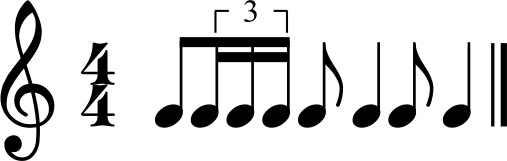
\includegraphics[scale=0.3]{img/subdivision_score1}\\
B & 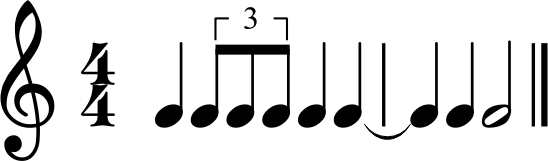
\includegraphics[scale=0.3]{img/subdivision_score2}\\
C & 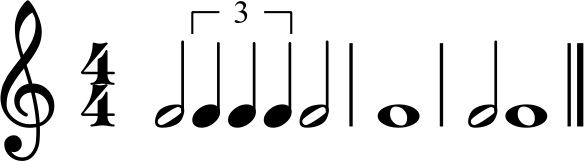
\includegraphics[scale=0.3]{img/subdivision_score3}\\
\hline
\end{tabular}
}
\caption{An analysis and three different score notations of the same musical clich\'e. }
\label{fig:subdivision}
\end{figure}

In modern staff notation the longest metrical unit is a whole note, which can be lengthened using dotted notation or ties. In the subdivision tree in figure \ref{fig:subdivision}, every node represents some metrical duration which may correspond to notes, bars or multiple bars. Although figure \ref{fig:subdivision} only shows duple and triple subdivisions, beats can be subdivided into any prime number of child-units. We specify two types of leaf-nodes: an onset, which we show as a $\bullet$ symbol in subdivision trees and a tied note, which we show as a $*$ symbol in subdivision trees. Figure \ref{fig:ties} shows how these symbols are interpreted. The $\propto$ symbol means that the expression on the left is equivalent to the expression on the right except for any global scaling of note durations.

\begin{figure}
\centering
\subfloat[A subdivision of a three note rhythm.]{
\parbox{0.25\linewidth}{
\centering
\Tree
[ .{$\frac{1}{1}$} [ .$\bullet$ ] [ .{$\frac{1}{2}$} [ .$\bullet$ ] [ .$\bullet$ ] ] ]
}
$\mathlarger{\mathlarger{\mathlarger{\propto}}}$
\parbox{0.25\linewidth}{
\centering
\includegraphics[scale=0.3]{img/intro1}
}
}

\subfloat[A subdivision tree of a two note rhythm containing a tied note.]{
\parbox{0.25\linewidth}{
\centering
\Tree
[ .{$\frac{1}{1}$} [ .$\bullet$ ] [ .{$\frac{1}{2}$} [ .$*$ ] [ .$\bullet$ ] ] ]
}
$\mathlarger{\mathlarger{\mathlarger{\propto}}}$
\parbox{0.25\linewidth}{
\centering
\includegraphics[scale=0.3]{img/intro2}
}
}
\caption{The interpretation of onsets and ties in subdivision trees.}
\label{fig:ties}
\end{figure}

The approach presented in \citet{longuet1976perception} is a rule-based system that needs to be initialised with a tactus interval and some tolerance parameter which specifies the rate at which the tempo is allowed to fluctuate. Nowadays, computers are powerful enough to construct probabilistic models based on corpora and to consider a great number of possible structural interpretations of a performance at once. With this in mind, we will briefly introduce our system below before discussing it in detail in the next chapter.

We will boil down a performance of a rhythm to a list of onsets. We think onsets provide enough information to correctly identify rhythmic structure. Therefore, we will from now on talk about onsets rather than notes.

Subdivision trees representing valid rhythmic structures can be described in a context-free grammar (CFG). An algorithm that determines the hierarchical structure of an input given some CFG is called a parser. We will present a CFG and a parser that constructs hierarchical structures like in figure \ref{fig:subdivision:a} from performances. Our parser will be some variant of a class of efficient parsing algorithms called chart-parsers.

Our parser will be guided by a Bayesian model which allows us to define a the probability of a rhythm given a performance as the probability of the rhythm itself, described by a \textit{rhythm model} times the probability that this rhythm generated the observed performance, described by an \textit{expression model}.

Similar to \cite{temperley2009unified}, we will use a rhythm model that is sensitive to common-practice notions about rhythm. However, instead of his hierarchical model, which is based on metrical grids, we will use a probabilistic context-free grammar (see section \ref{sec:prior}). This model follows naturally from our representation of rhythmic structure. In chapter \ref{sec:discussion}, we will evaluate how the PCFG prior compares to the hierarchical model.

We have claimed that some expressive deviations may have some structure-related regularities. Emphasising beats can result in a slight stretching of the duration of the beat. Depending on the style of the music, some beats may be emphasised consistently. It is often said that downbeats are emphasised in many music styles. If this does indeed lead to stretching them, it will result in downbeats at levels near the leaf nodes of the tree to be slightly longer than upbeats. A tempo independent way to look at this is as the ratio of downbeat length and upbeat length. Our expression model will assume that the down-/upbeat length ratio can be estimated from a small feature set.

To train our rhythm and expression model, we need a corpus of monophonic performances annotated with subdivision trees. There are, as far as we know, very few corpora available where expressively performed music is annotated with metrical structure and there are no corpora where this structure is represented as subdivision trees. There is a publicly available corpus of classical piano music performances of very high quality, annotated with tempo and deviation information for every performed note \citep{hashida2008new}. There are similar corpora in existence, notably one containing performances of Chopin by Nikita Magaloff \citep{flossmann2010magaloff}, but these are not publicly available due to issues with copyright. 

So although there is one freely available corpus, this corpus covers classical music. We think that we are more likely to find some form of regular expressive deviation in music that is generally performed at a relatively constant tempo. Jazz music seems to fit this requirement. As far as we know, there are no freely available corpora of jazz music annotated with rhythmic structure and therefore we endeavoured to create our own corpus.

The corpus we constructed contains monophonic jazz melodies, performed by amateur musicians. The corpus was annotated with metrical onset times and subdivision trees were generated using a non-probabilistic version of our parser. This was possible because we could assume the onset times were metronomic.\footnote{Technically, the onsets are specified in metrical units and not metronomic units. However, since our parser is tempo-independent this does not matter.}

We will evaluate the parser on the jazz corpus. Since we do not have enough data to keep a separate test set, we have to use cross-validation. This means that we are effectively testing on our development set.
%Representation: subdivision trees
%Context free grammar, parser
%Bayesian model: rhythm model, expression model
%Parameters learned from annotated corpus.
%Expression model: expression ratio
%Advantage of subdivision trees with respect to expression: we always know what the down- and upbeats are.